\documentclass[10.5pt]{report}

% Used Packages
\usepackage{xeCJK} % Chinese Language Settings
\usepackage{fontspec}
\setCJKmainfont{Source Han Serif SC}
\setmainfont{Minion Pro}

\usepackage{indentfirst}  % indent of Chinese
\setlength{\parindent}{2em}

\setlength{\parskip}{0.5em}

\usepackage{lmodern} %Math Settings
\usepackage{amssymb,amsmath}
\usepackage{unicode-math}
\setmathfont{Asana-Math}
\defaultfontfeatures{Scale=MatchLowercase}

\usepackage{color} 
\usepackage[table,xcdraw]{xcolor} % color of column

\usepackage{soulutf8}
\usepackage{hyperref} %hyperref fot TOC
\hypersetup{
	colorlinks=true,
	linkcolor=black, % black for TOC
	filecolor=magenta,      
	urlcolor=blue, % blue for URL
}
\usepackage{pdfpages} 
\usepackage{graphicx}

\usepackage{geometry} % set margin
 \geometry{
	a4paper,
	total={170mm,257mm},
	left=20mm,
	top=25mm,
}

\usepackage{longtable} %for multi columns alignment (eg. Name & Ins.)
\usepackage{booktabs}%for line in longtable
\usepackage{setspace} % for setting space between two line
\renewcommand{\baselinestretch}{1.2}

\usepackage{chemfig} %for chemistry formulae
\usepackage{multirow} % for multi-row table




% User defined command or settings
\newcommand{\mychapter}[1]{
	\chapter*{#1}
	\addcontentsline{toc}{chapter}{#1}
}
\newcommand{\mysection}[1]{
	\section*{#1}
	\addcontentsline{toc}{section}{#1}
}% these two commands removed the number of chapters/sections in contents
\renewcommand{\contentsname}{目录} % change name of contents


\title{52\textsuperscript{th} ICHO预备题中文翻译}
\author{ICHO预备题中文翻译组}
\date{\today} 
\begin{document}                     
\maketitle                              % Print title page.
\newpage
\pagenumbering{roman}          
\setcounter{page}{2}                    % make it start with "ii"
\section*{翻译说明}
很高兴可以为大家提供第52届IChO预备题的中文翻译稿,该译稿基于2020年1月31日发布的原版第一版,我们在翻译过程中已尽可能仔细地审阅过试题(也修正了一些显而易见的错误),但仍可能存在一些难以发现的问题。限于时间与精力,我们不太可能会继续更新新的翻译版本。为确保题目的正确性,请读者自行访问官方网站,查看最新的官方勘误。

官方网站:\href{https://https://icho2020.tubitak.gov.tr/icho-2020-hazirlik-sorular%C4%B1}{https://icho2020.tubitak.gov.tr/icho-2020-hazirlik-soruları}

本译稿采用知识共享署名–非商业性使用–相同方式共享 3.0 中国大陆许可协议进行许可。全体译稿作者保留追究此协议及相关法律许可内的一切权利。\\

\noindent \textbf{翻译人员名单(按拼音顺序排列)}

\textbf{翻译:}


\begin{longtable}{ p{2cm}p{12cm} } % choose suitable width for "p" column
abc&清华大学\\
efg&北京大学\\

\end{longtable}
\textbf{图片:}

\begin{longtable}{ p{2cm}p{12cm}}  % choose suitable width for "p" column
abc&清华大学\\
efg&北京大学\\
\end{longtable}
\textbf{校对:}

\begin{longtable}{p{2cm}p{12cm} }  % choose suitable width for "p" column
abc&清华大学\\
efg&北京大学\\
\end{longtable}
\textbf{排版:}

\begin{longtable}{p{2cm}p{12cm} }  % choose suitable width for "p" column
abc&清华大学\\
efg&北京大学\\
	\LaTeX
\end{longtable}

\newpage
\section*{前言}
我们非常高兴为将于2020年在土耳其伊斯坦布尔举行的第52届国际化学奥林匹克竞赛提供预备题。 我们准备了这些问题,旨在促进参与者的培训和准备。我们 精心选择了问题的内容,以涵盖现代化学和经典化学中可能遇到的一系列具有挑战性的主题。 这些问题可以通过应用高中化学的基本原理以及理论部分的6个高级难度主题和实践部分的3个高级难度主题来解决。 这些高级主题明确列在“高级难度主题”下,并且在试题中演示了它们的应用。 我们希望参与者熟悉这些高级主题。

本手册中列出的问题包括25个理论试题和8个实验试题。 答案将在2020年3月1日之前通过电子邮件发送到每个国家的首席指导官,并在2020年5月15日之前在我们的IChO 2020网站上发布。 我们欢迎您对\href{icho2020@tubitak.gov.tr}{icho2020@tubitak.gov.tr} 提出任何意见,建议,更正或疑问。

国际化学奥林匹克提供了一个很好的机会,激发年轻一代从事基础科学事业,并对公众对科学尤其是化学的态度产生积极影响。 我们希望您会喜欢解决这些问题,并期待与您在7月的土耳其伊斯坦布尔见面。

\section*{致谢}

我要感谢所有作者为筹备问题做出的奉献和努力,以及国际指导委员会成员的宝贵意见和建议,深表感谢。 我们还高度赞赏土耳其科学技术研究委员会(TUBITAK)与伊斯坦布尔科技大学(ITU)理学院合作,为IChO 2020之前和期间的所有组织工作提供便利。\\

\noindent
代表科学委员会

\noindent
\textbf{Dr. Arif DASTAN}
\newpage

\tableofcontents                        % Print table of contents

\newpage
\mysection{作者}
\noindent 	
ALANYALIOĞLU, Murat, \emph{Atatürk University}\\
ARSLAN, Yasin, \emph{Burdur Mehmet Akif Ersoy University}\\
AYDOĞAN, Abdullah, \emph{İstanbul Technical University}\\
BOZKAYA, Uğur, \emph{Hacettepe University} \\
BURAT, Ayfer Kalkan, \emph{İstanbul Technical University}\\
DAĞ, Ömer, \emph{Bilkent University}\\
DAŞTAN, Arif, \emph{Atatürk University (\textbf{Chair of Scientific Committee})}\\
ELTUĞRAL, Nurettin, \emph{Karabük University}\\
GÖLCÜ, Ayşegül, \emph{İstanbul Technical University}\\
KANBUR, Yasin, \emph{Karabük University}\\
KILIÇ, Hamdullah, \emph{Atatürk University}\\
METİN, Önder, \emph{Koç University}\\
SARAÇOĞLU, Nurullah, \emph{Atatürk University}\\
TÜRKMEN, Yunus Emre, \emph{Bilkent University}\\
ÜNLÜ, Caner, \emph{İstanbul Technical University}\\
YILMAZ, İsmail, \emph{İstanbul Technical University}\\

\noindent
\textbf{编辑:}\\
SARAÇOĞLU, Nurullah, \emph{Atatürk University}\\

\newpage
\mysection{物理常数与方程}

\setlength{\parskip}{0em}

Avogadro常数:$N_A=6.0221\times10^{23}\ \mathrm{mol}^{-1}$

Boltzmann常数:$k_B=1.3807\times10^{-23}\ \mathrm{J\ K}^{-1}$

普适气体常数:$R=8.3145\ \mathrm{J\ K^{-1}\ mol^{-1}} = 0.08205\ \mathrm{atm\ L\ K^{-1}\ mol^{-1}}$

光速:$c=2.9979\times10^8\ \mathrm{m\ s^{-1}}$

Planck常数:$h=6.6261\times10^{-34}\ \mathrm{J\ s}$

Faraday常数:$F=9.6485\times10^4\ \mathrm{C\ mol^{-1}}$

电子质量:$m_e=9.10938215\times10^{-31}\ \mathrm{kg}$

标准气压:$P=1\ \mathrm{bar}=10^5\ \mathrm{Pa}$

大气压:$P_{\mathrm{atm}}=1.01325\time10^5\ \mathrm{Pa}=760\ \mathrm{mmHg}=760\ \mathrm{torr}$

摄氏零度:$273.15\ \mathrm K$

$1\ \mathrm{pm}=10^-12\ \mathrm m$; $1 Å = 10^{-10}\ \mathrm m$; $1\ \mathrm{nm} = 10^{-9}\ \mathrm m$

$1\ \mathrm{eV}=1.6\times10^-19\ \mathrm J$

$1\ \mathrm{cal}=4.184\ \mathrm J$

$1\ \mathrm{aum}=1.66053904\times10^{-27}\ \mathrm{kg}$

\begin{longtable}{ p{3.2cm}p{12cm} } % choose suitable width for "p" column
电子电荷:&$1.6\times10^{-19}\mathrm C$\\
理想气体方程:&$pV=nRT$\\
焓:&$H=U+pV$\\
Gibbs自由能:&$G=H-TS$\\
&$\Delta G=\Delta G^\ominus+RT\ln Q$\\
&$\Delta G^{\ominus}=-RT\ln K=-nFE_{\mathrm{cell}}^\ominus$\\
熵变:&$\Delta S=\frac{q_{\mathrm{rev}}}{T}$,其中$q_{\mathrm{rev}}$是可逆过程的热\\
&$\Delta S=nRT\ln\frac{V_2}{V_1}$(理想气体绝热膨胀)\\
Nernst方程:&$E=E^\ominus+\frac{RT}{nF}\ln\frac{c_{\mathrm{ox}}}{c_{\mathrm{red}}}$\\
光子能量:&$E=\frac{hc}{\lambda}$\\
速率方程 &\\
零级:&$[A]=[A]_0-kt$\\
一级:&$\ln[A]=\ln[A]_0-kt$\\
二级:&$\frac{1}{[A]}=\frac{1}{[A]_0}+kt$\\
Arrhenius方程:&$k=Ae^{-E_a/RT}$\\
线性回归:&$y=mx+n$\\
标准差:&$s=\sqrt{\frac{\sum_{x=1}^N (x_1-\bar x)^2}{N-1}}$\\
Lambert-Beer方程:&$A=\varepsilon lc$
\end{longtable}
\setlength{\parskip}{0.5em}

\newpage
\mysection{元素周期表}
Table


\newpage
\mysection{\texorpdfstring{\textsuperscript{1}}{TEXT}H NMR化学位移}
111

\newpage
\mysection{典型的耦合常数}
111

\newpage
\mysection{\texorpdfstring{\textsuperscript{13}}{TEXT}C NMR化学位移}
111

\newpage
\mysection{红外频率吸收表}
\begin{longtable}[]{@{}llll@{}}
	\toprule
	\endhead
	\textbf{官能团} & \textbf{振动类型} &
	\textbf{吸收频率(cm\textsuperscript{--1})} &
	\textbf{强度}\tabularnewline
	\textbf{醇} & & &\tabularnewline
	O--H & (伸缩, H--键合的) & 3600--3200 & 强,宽\tabularnewline
	& (伸缩, 自由的) & 3700--3500 & 强,尖\tabularnewline
	C--O & (伸缩) & 1150--1050 & 强\tabularnewline
	\textbf{烷烃} & & &\tabularnewline
	C--H & 伸缩 & 3000--2850 & 强\tabularnewline
	& 弯曲 & 1480--1350 & 可变的\tabularnewline
	\textbf{烯烃} & & &\tabularnewline
	=C--H & 伸缩 & 3100--3010 & 中等\tabularnewline
	& 弯曲 & 1000--675 & 强\tabularnewline
	C=C & 伸缩 & 1680--1620 & 可变的\tabularnewline
	\textbf{烷基卤} & & &\tabularnewline
	C--F & 伸缩 & 1400--1000 & 强\tabularnewline
	C--Cl & 伸缩 & 800--600 & 强\tabularnewline
	C--Br & 伸缩 & 600--500 & 强\tabularnewline
	C--I & 伸缩 & 500 & 强\tabularnewline
	\textbf{炔烃} & & &\tabularnewline
	C--H & 伸缩 & 3300 & 强, 尖\tabularnewline
	C≡C&伸缩&2260--2100&可变的, 对称炔没有\tabularnewline
	\textbf{胺} & & &\tabularnewline
	N--H & 伸缩 & 3500--3300 & 伯胺有两个带,中等\tabularnewline
	&&&仲胺有一个带,非常弱	\tabularnewline
	C--N & 伸缩 & 1360--1080 & 中等-弱\tabularnewline
	N--H & 弯曲 & 1600 & 中等\tabularnewline
	\textbf{芳香的} & & &\tabularnewline
	C--H & 伸缩 & 3100--3000 & 中等\tabularnewline
	C=C & 伸缩 & 1600--1400 & 中等-弱,多个带\tabularnewline
	\textbf{羰基} & & &\tabularnewline
	C=O & 伸缩 & 1820--1670 & 强\tabularnewline
	\textbf{羧酸} & & &\tabularnewline
	C=O & 伸缩 & 1725--1700 & 强\tabularnewline
	O--H & 伸缩 & 3300--2500 & 强,非常宽\tabularnewline
	C--O & 伸缩 & 1320--1210 & 强\tabularnewline
	\textbf{醛} & & &\tabularnewline
	C=O & 伸缩 & 1740--1720 & 强\tabularnewline
	C--H & 伸缩 & 2850--2820 \& 2750--2720 & 中等,两个峰\tabularnewline
	\textbf{酰胺} & & &\tabularnewline
	C=O & 伸缩 & 1690--1640 & 强\tabularnewline
	N--H & 伸缩 & 3500--3100 & 未取代的有两个带\tabularnewline
	& 弯曲 & 1640--1550 &\tabularnewline
	\textbf{酸酐} & & &\tabularnewline
	C=O & 伸缩 & 1830--1800 \&1775--1740 & 两个带\tabularnewline
	\textbf{酯} & & &\tabularnewline
	C=O & 伸缩 & 1750--1735 & 强\tabularnewline
	C--O & 伸缩 & 1300--1000 & 两个或多个带\tabularnewline
	\textbf{酮} & & &\tabularnewline
	非环状 & 伸缩 & 1725--1705 & 强\tabularnewline
	环状 & 伸缩 & 3-元环 - 1850 & 强\tabularnewline
	& 伸缩 & 4-元环 - 1780 & 强\tabularnewline
	& 伸缩 & 5-元环 - 1745 & 强\tabularnewline
	& 伸缩 & 6-元环 - 1715 & 强\tabularnewline
	& 伸缩 & 7-元环 - 1705 & 强\tabularnewline
	$\alpha,\beta$-不饱和的& 伸缩 & 1685--1665 & 强\tabularnewline
	芳基酮& 伸缩 & 1700--1680 & 强\tabularnewline
	\textbf{醚} & & &\tabularnewline
	C--O & 伸缩 & 1300--1000 (1150--1070) & 强\tabularnewline
	\textbf{腈} & & &\tabularnewline
	C≡N & 伸缩 & 2260--2210 & 中等\tabularnewline
	\textbf{硝基} & & &\tabularnewline
	N--O & 伸缩 & 1560--1515 \& 1385--1345 & 强,两个带\tabularnewline
	\bottomrule
\end{longtable}

\newpage
\mysection{高级难点}
\noindent \textbf{理论部分}
\begin{enumerate}
 	\item 周环反应(环加成和电环化反应)。
 	\item \emph{sp}\textsuperscript{2}碳中心的亲核取代反应。
 	\item 光谱:基本的\textsuperscript{1}H和\textsuperscript{13}C	NMR谱(化学位移,信号多重性,强度和耦合常数); 简单的红外光谱。
 	\item 动力学:速率常数模型和动力学同位素效应。
 	\item 基本量子化学:电子能级,应用于共轭体系的跃迁,分子的振动和旋转运动(提供公式),以及共轭 体系的简单理论。
 	\item 无机化学:同/异核双原子分子的配位化学(晶体结构,晶体场论和异构现象)和分子轨道能图。
 \end{enumerate}

\noindent
\textbf{注意:}

i) 下列主题不会在考试中出现

\begin{itemize}
	\item 金属催化的交叉偶联反应和烯烃复分解反应。
	\item 使用Microsoft Excel或任何相关的计算机软件。
	\item 使用导数和积分。
	\item 尽管预备问题中的一些例子与生物分子有关,但不应要求学生将任何生物化学或碳水化合物化学作为高级主题。
	\item 无机反应机理。
	\item 多原子分子的分子轨道图。
\end{itemize}

ii) 除非重要,否则反应流程中的箭头不会显示反应条件,例如溶剂和温度。\\

\noindent
\textbf{实验部分}

\begin{enumerate}
	\item 使用分光光度计(单/双波长测量)。
	\item 有机合成中的基本技术:重结晶,薄层色谱法(TLC),过滤和按照所描述的程序干燥沉淀物。
	\item 蒸馏和萃取。
\end{enumerate}

\noindent
\textbf{注意:}
下列主题不会在考试中出现

\begin{itemize}
	\item 确定熔点。
	\item 使用旋转蒸发仪。
	\item 处理和处理对水分敏感的化合物(使用注射器和气球)。
	\item 进行柱层析。
	\item 实验中通过聚合产生水凝胶体系。
\end{itemize}


\mychapter{理论试题}
\pagenumbering{arabic}

\mysection{第1题\ 丁二烯的 \texorpdfstring{$\pi$} {TEXT}电子体系}

test

\newpage
\mysection{第25题\  分光光度法测定抗组胺药}

分光光度法是用于确定药物分子的简单,快速和准确的方法。该方法基于两种试剂之间形成复合物。许多复合物是有色的,并在可见光区域有吸收。因此可以用分光光度法测定它们。

抗组胺药物\textbf{D}作为给电子基团,与$\pi$-受体\textbf{S}复合。所得的复合物在最大吸收(460 nm)处记录的吸光度与药物浓度线性相关,具有良好的相关系数。
$$
\begin{aligned}
\mathrm D+\mathrm S\rightleftharpoons\mathrm {DS}\\
K=\frac{[\mathrm{DS}]}{[\mathrm D][\mathrm S]}\\
\end{aligned}
$$
其中\([\mathrm{DS}]\),\([\mathrm D]\)与\([\mathrm S]\)分别代表\textbf{DS}复合物,\textbf{D}与\textbf{S}的平衡浓度。
\[
c_{\mathrm D}=[\mathrm D]+[\mathrm {DS}]
\] 
其中\(c_{\mathrm D}\)是药物的总浓度。

只有所形成的\textbf{DS}络合物可以吸收光的波长下,以下表达式成立:

 \[
A=\varepsilon_{\mathrm{DS}}l[\mathrm{DS}]
\] 
其中\(l\)是吸收池长度。

可以使用Benesi--Hildebrand方程来计算络合物的结合平衡常数,该方程取决于实验条件,其中一种组分应大量过量,以使其浓度不会随复合物的形成而改变。

\[
\frac{c_{\mathrm D}}{A_{\mathrm{DS}}}=\frac{1}{\varepsilon_{\mathrm{DS}}}+\frac{1}{\varepsilon_{\mathrm{DS}}K}\times\frac{1}{c_{\mathrm S}}
\]
其中\(c_{\mathrm S}\)与\(c_{\mathrm D}\)是\textbf{S}与\textbf{D}的总浓度。\(A_{\mathrm{DS}}\)是复合物的吸光度,\(\varepsilon_{\mathrm{DS}}\)是复合物的摩尔吸光系数,\(K\)是平衡常数。

\begin{figure}[h]
	\centering
	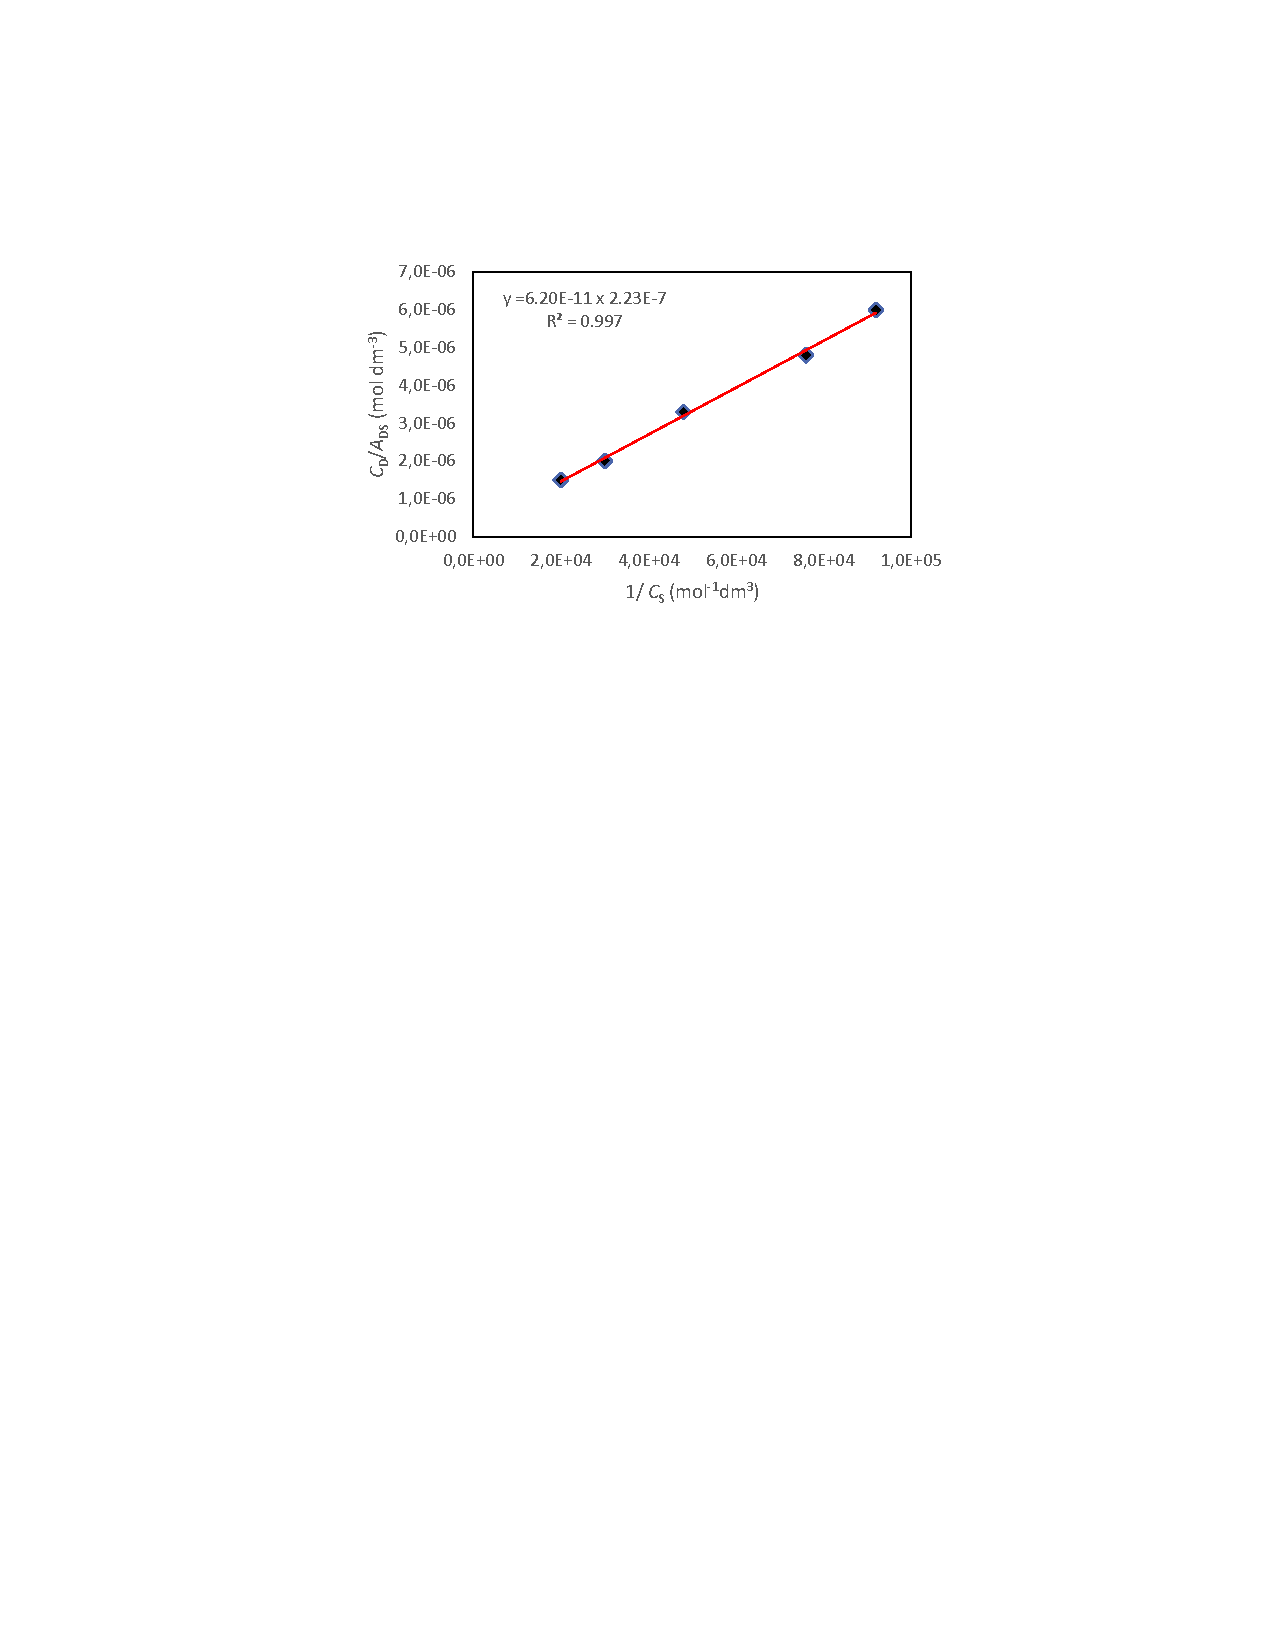
\includegraphics[width=12cm]{./pic/t25-1.pdf}
\end{figure}

\noindent\textbf{25.1.} 考虑在25
°C下记录的Benesi--Hildebrand图,给出复合物生成的平衡常数和复合物的摩尔吸光系数。


\noindent\textbf{25.2.}
\textbf{D}与\textbf{S}的起始浓度是9×10\textsuperscript{−5} mol
L\textsuperscript{−1},计算平衡时复合物形成的百分数。\textbf{D}与\textbf{S}在复合的时候比例为1:1。

\noindent\textbf{25.3.} 计算25 °C下的\(\Delta_rG^\ominus\),单位为kJ
mol\textsuperscript{−1}。

通过改变温度(25、45和60 °C)研究\textbf{D}与\textbf{S}的络合动力学。该表给出了在不同温度下的络合速率常数。

\begin{longtable}[]{@{}llll@{}}
	\toprule
	$T$ (°C) &25&45&60 \tabularnewline
	$k$ (min\textsuperscript{--1}) & 0.0200 &0.0504&0.0944\tabularnewline
	\bottomrule
\end{longtable}

\noindent\textbf{25.4.} 计算活化能\(E_a\)。

\noindent\textbf{25.5.}
已知\(k_{\mathrm{TST}}=\frac{k_{\mathrm BT}}{h}e^{-\frac{\Delta G^\ddag}{RT}}\),计算25 °C下的活化焓\(\Delta H^\ddag\),活化熵\(\Delta S^\ddag\)以及活化自由能\(\Delta G^\ddag\)。
(译注:原文为自由活化焓\(\Delta G^\ddag\))



\mychapter{实验试题}


\end{document}                          % The required last line